\documentclass[11pt,compress,t,notes=noshow, aspectratio=169, xcolor=table]{beamer}

\usepackage{../../style/lmu-lecture}
% Defines macros and environments
% This file is included in slides and exercises

% Rarely used fontstyle for R packages, used only in 
% - forests/slides-forests-benchmark.tex
% - exercises/single-exercises/methods_l_1.Rnw
% - slides/cart/attic/slides_extra_trees.Rnw
\newcommand{\pkg}[1]{{\fontseries{b}\selectfont #1}}

% Spacing helpers, used often (mostly in exercises for \dlz)
\newcommand{\lz}{\vspace{0.5cm}} % vertical space (used often in slides)
\newcommand{\dlz}{\vspace{1cm}}  % double vertical space (used often in exercises, never in slides)
\newcommand{\oneliner}[1] % Oneliner for important statements, used e.g. in iml, algods
{\begin{block}{}\begin{center}\begin{Large}#1\end{Large}\end{center}\end{block}}

% Don't know if this is used or needed, remove?
% textcolor that works in mathmode
% https://tex.stackexchange.com/a/261480
% Used e.g. in forests/slides-forests-bagging.tex
% [...] \textcolor{blue}{\tfrac{1}{M}\sum^M_{m} [...]
% \makeatletter
% \renewcommand*{\@textcolor}[3]{%
%   \protect\leavevmode
%   \begingroup
%     \color#1{#2}#3%
%   \endgroup
% }
% \makeatother


\title{Interpretable Machine Learning}
% \author{LMU}
%\institute{\href{https://compstat-lmu.github.io/lecture_iml/}{compstat-lmu.github.io/lecture\_iml}}
\date{}

\begin{document}

\newcommand{\titlefigure}{figure/logreg-2vars-surface}%{figure/logistic_marginal_temp.pdf}
\newcommand{\learninggoals}{
\item Definition of GLMs
\item Logistic regression as example
\item Interpretation in logistic regression
}

\lecturechapter{Generalized Linear Models}
\lecture{Interpretable Machine Learning}


%------------------------------------------------------------------
%------------------------------------------------------------------
\begin{frame}{Generalized Linear Model (GLM) \citebutton{Nelder and Wedderburn 1972}{https://doi.org/10.2307/2344614}}
\vspace{-0.2cm}
\textbf{Problem}: Target variable given feat. not always normally dist. $\leadsto$ LM not suitable
\begin{itemize}
    \item Target is binary (e.g., disease classification)\\
    $\leadsto$ Bernoulli / Binomial distribution
\end{itemize}
\vspace{-0.5cm}
\begin{columns}[totalwidth=\textwidth]
    \begin{column}{0.45\textwidth}
        \begin{itemize}
            \item Target is count variable \\(e.g., number of sold products)\\
            $\leadsto$ Poisson distribution
            \item Time until an event occurs\\ (e.g., time until death)\\
            $\leadsto$ Gamma distribution
        \end{itemize}
    \end{column}
    \begin{column}{0.55\textwidth}
    \vspace{-0.4cm}
        \begin{center}
            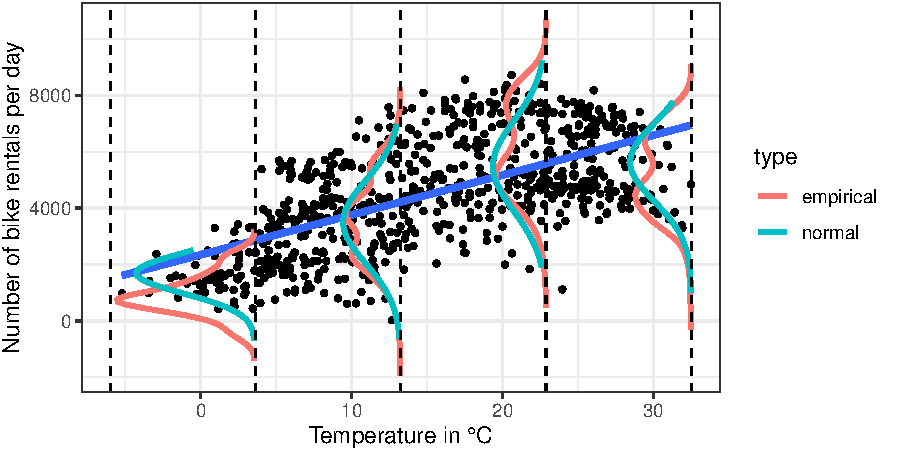
\includegraphics[width = 0.9\textwidth]{figure/density_intervals.pdf}
        \end{center}
    \end{column}
\end{columns}
\medskip
\pause
\textbf{Solution}: GLMs - extend LMs by allowing other distributions from exponential family
%$$g(\E (y \mid \xv)) = \theta_0 + \theta_1 x_1 + \theta_2 x_2 + \ldots + \theta_p x_p$$
% \begin{align*}
% &g(\E (y \mid \xv)) = 
% %\theta_0 + \theta_1 x_1 + \theta_2 x_2 + \ldots + \theta_p x_p = 
% \xv^\top \theta\\
% \Leftrightarrow \; & \E (y \mid \xv) = g^{-1}(\xv^\top \theta)
% \end{align*}
$$g(\E (y \mid \xv)) = \xv^\top \theta \; \Leftrightarrow \; \E (y \mid \xv) = g^{-1}(\xv^\top \theta)$$
\vspace*{-0.5cm}
    \begin{itemize}
        \item Link function $g$ links linear predictor $\xv^\top \theta$ to expectation of distribution of $y \mid \xv$\\ %$\E$ of specified distribution of
        $\leadsto$ LM is special case: Gaussian distribution for $y \mid \xv$ with $g$ as identity function 
        \item Link function $g$ and distribution need to be specified 
        \item High-order and interaction effects can be manually added as in LMs
        \item Note: Interpretation of weights depend on link function and distribution
    \end{itemize}
 %   \medskip
 %   Non-Gaussian outputs via Generalized Linear Models (GLMs):
  %  \begin{itemize}
   %     \item link function $g$ -- can be freely chosen
    %    \item exponential family defining $\E_Y$ -- can be freely chosen
     %   \item weighted sum $X^\top W$
    %\end{itemize}
    %\medskip 
    %\pause
    %Interaction effects via feature engineering:
    %\begin{itemize}
    %    \item E.g., feature expansion: $\theta_{x_i,x_j} x_i \cdot x_j$
    %\end{itemize}
\end{frame}
 	
\begin{frame}{GLM - Logistic Regression}
%\begin{columns}[T, totalwidth=\textwidth]
%\begin{column}{0.45\textwidth}

\begin{itemize}
    \item Logistic regression $\hat{=}$ GLM with Bernoulli distribution and logit link function: 

\begin{align*}
    g(x) &= \log\left(\frac{x}{1 - x}\right)  
    \Rightarrow \; g^{-1}(x) &= \frac{1}{1+\exp(-x)}
\end{align*}
%\end{column}
%\begin{column}{0.55\textwidth}

% \begin{columns}[c, totalwidth=\textwidth]
% \begin{column}{0.005\linewidth}
% \scriptsize
% \rotatebox[origin=c]{90}{\hspace{10pt}$P(y = 1)$}
% \end{column}
% \begin{column}{0.995\linewidth}
%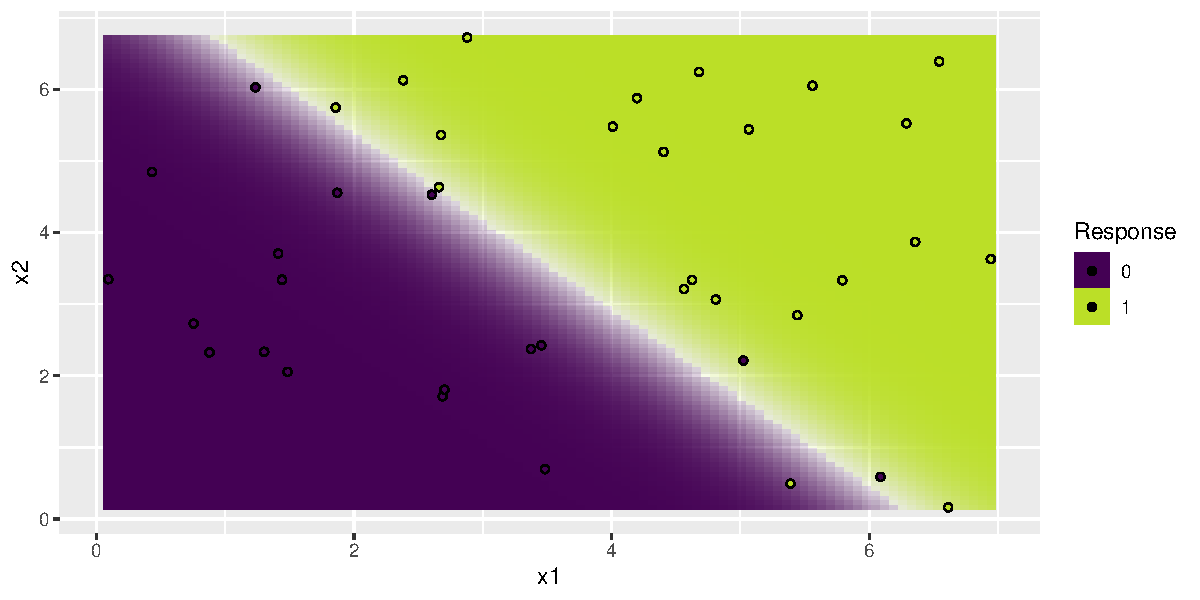
\includegraphics[width = \textwidth]{figure/reg_class_log_6.pdf}
% \scriptsize\centerline{$\xv^\top \theta$}
% \end{column}
% \end{columns}
%\end{column}
%\end{columns}

%\bigskip

% \begin{columns}[T, totalwidth=\textwidth]
% \begin{column}{0.65\textwidth}
% \begin{itemize}
    \item Models probabilities for binary classification by
    $$\pi(\xv) = \E(y \mid \xv) = P(y = 1) = g^{-1}(\xv^\top \theta) = \frac{1}{1 + \exp(- \xv^\top \theta)} $$
    %\item Logistic regression models $\E(y \mid \xv) = P(y = 1)$, i.e., probabilities for binary classification 
    %\item Logistic regression formula:
    %$$P(y = 1) =\frac{1}{1 + \exp(-( \theta_0 + \theta_1 x_1 + \theta_2 x_2 + \ldots + \theta_p x_p ))} $$
\end{itemize}
% \end{column}
% \begin{column}{0.35\textwidth}
% \end{column}
% \end{columns}
\centering
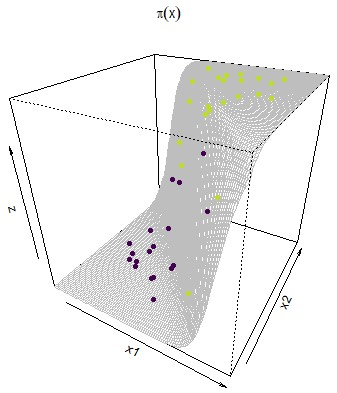
\includegraphics[width=0.3\textwidth]{figure/logreg-2vars-surface.png} \qquad
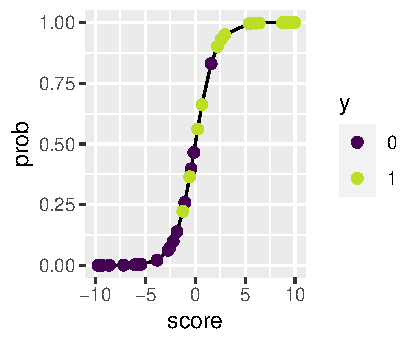
\includegraphics[width=0.4\textwidth]{figure/reg_class_log_7} 
\end{frame}



\begin{frame}{GLM - Logistic Regression}

\begin{itemize}
    \item Typically, we set the threshold to $0.5$ to predict classes, e.g.,
    \begin{itemize}
        \item Class 1 if $\pi(\xv) > 0.5$
        \item Class 0 if $\pi(\xv) \leq 0.5$
    \end{itemize}
\end{itemize}

\medskip
\centering
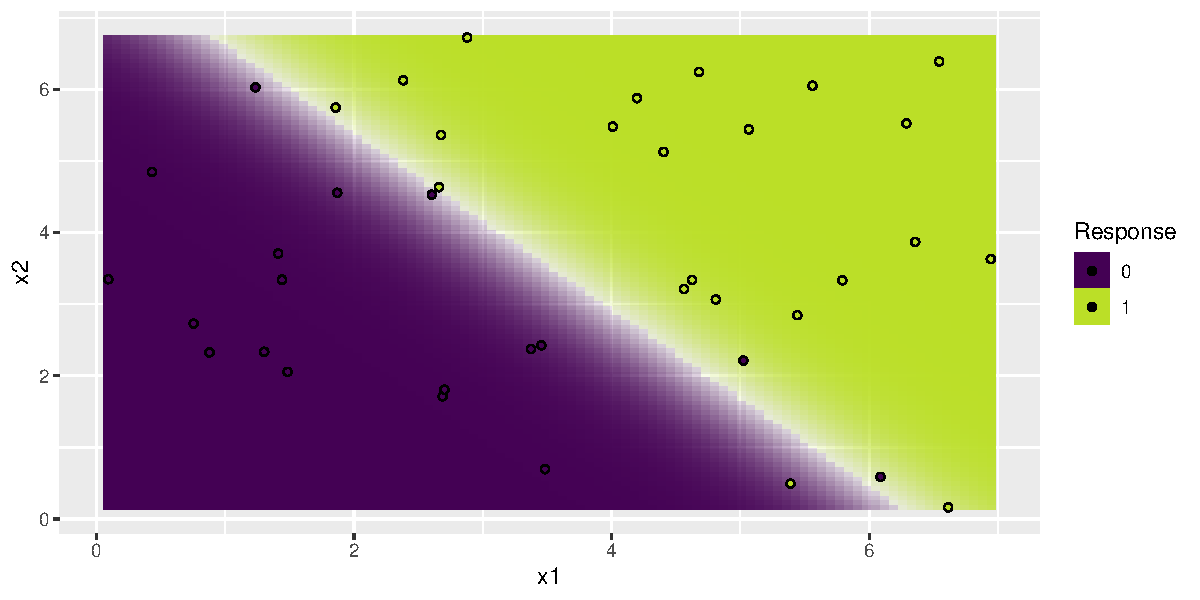
\includegraphics[width = \textwidth]{figure/reg_class_log_6.pdf}
% figs from i2ml course, Chapter 03.04: Logistic Regression, slide 7 
\end{frame}


% \begin{frame}{Generalized Linear Models (GLMs)}

% \begin{align*}
% g\left(\mathbb{E}_Y(Y \vert X)\right) &= X^T\theta \\
% \mathbb{E}_Y \left(Y \vert X\right) &= g^{-1}(X^T\theta)
% \end{align*}
% \begin{itemize}[<+->]
% %\setlength\itemsep{1em}
% %\item GLMs are a framework for target distributions of  exponential families (e.g., Gaussian, Binomial, Poisson, Gamma). Gaussian target distribution $+$ identity link $\hat =$ linear / polynomial model.
% \item GLM framework assumes distribution of $Y$ is a member of exponential families, e.g.: % (e.g., Gaussian, Binomial, Poisson)
% \begin{itemize}[<.->]
%     \item Gaussian target distribution $+$ identity link $\hat =$ linear / polynomial model.
%     \item Binomial target distribution $+$ logit link $log\left(\frac{\mathbb{E}_Y(Y \vert X)}{1 - \mathbb{E}_Y(Y \vert X)}\right)$ $\hat =$ logistic regression.
% \end{itemize}
% %\item GLMs keeps linear predictor $X^T\theta$ (explains $\mathbb{E}_Y(Y \vert X)$ through a more flexible link function $g$).
% \item Link function $g$ describes how $X^T\theta$ relates to the expected, conditional target $\mathbb{E}_Y(Y \vert X)$.
% \begin{itemize}[<.->]
%     \item Interpretations as for linear / polynomial models but w.r.t. transformed target via $g$.
%     \item Linear terms become non-linear through the link function (except for identity link)!
% \end{itemize}
% %\item If the target is distributed binomially, a natural link function is the logit link $log\left(\frac{\mathbb{E}_Y(Y \vert X)}{1 - \mathbb{E}_Y(Y \vert X)}\right)$ (logistic regression).
% \item We need to specify the correct model equation, target distribution, and link function to receive a good model fit.
% %\item %As the model equation is still known, interpretations are possible the same way as for polynomial regression models.
% %However, even linear terms become non-linear through the link function (if the identity link is not used)!
% \end{itemize}
% \end{frame}
%------------------------------------------------------------------
%------------------------------------------------------------------

\begin{frame}[c]{GLM - Logistic Regression - Interpretation}

    \begin{itemize}
        \item \textbf{Recall:} Odds is ratio of two probabilities, odds ratio compares ratio of two odds 
        \item Weights $\theta_j$ are interpreted linear as in LM (but w.r.t. log-odds) \\
        $\leadsto$ difficult to comprehend
        %relate to log-odds %$\leadsto$ Effects are linear as in LM (but w.r.t. log-odds)
        $$log\text{-}odds = \log \left(\frac{\pi(\xv)}{1 - \pi(\xv)}\right) = \log \left(\frac{P(y=1)}{P(y=0)}\right) = \theta_0 + \theta_1 x_1 + \ldots + \theta_p x_p  $$
        \textbf{Interpretation:} \\ Changing $x_j$ by one unit, changes log-odds of class 1 compared to class 0 by $\theta_j$%\\
        %$\leadsto$ Effects are interpreted linear as in LM (but w.r.t. log-odds) $\leadsto$ difficult to comprehend
        \pause
        \item Odds for class 1 vs. class 0: %Odds can be caulculated by:
        $odds = \displaystyle\frac{\pi(\xv)}{1 - \pi(\xv)}= \exp(\theta_0 + \theta_1 x_1 + \ldots + \theta_p x_p)$
        \item Instead of interpreting changes w.r.t. log-odds,  $odds\text{ }ratio$ is more common
        $$ = \frac{odds_{x_j+1}}{odds} = \frac{\exp(\theta_0 + \theta_1 x_1 + \ldots + \theta_j (x_j+1) + \ldots + \theta_p x_p)}{\exp(\theta_0 + \theta_1 x_1 + \ldots + \theta_j x_j + \ldots + \theta_p x_p)} = \exp{(\theta_j)} $$
        \textbf{Interpretation}: Changing $x_j$ by one unit, changes the \textbf{odds ratio} for class 1 (compared to class 0) by the \textbf{factor} $\exp(\theta_j)$
        %\pause
        %\item Interpretation for different feature types is the same as for linear regression (however, linear interpretation only possible w.r.t. log odds $\leadsto$ difficult to comprehend)
    \end{itemize}	

\end{frame}

\begin{frame}{GLM - Logistic Regression - Example}

\begin{itemize}
    \item Create a binary target variable for bike rental data:
    \begin{itemize}
        \item Class 1: ``high number of bike rentals'' $>70\%$ quantile (i.e., \code{cnt} $> 5531$)
        \item Class 0: ``low to medium number of bike rentals'' (i.e., \code{cnt} $\leq$ 5531)
    \end{itemize}
    \item Fit a logistic regression model (GLM with Bernoulli distribution and logit link)
\end{itemize}

\begin{columns}[T, totalwidth = \textwidth]
\begin{column}{0.55\textwidth}
%\begin{table}[ht]
\centering
% \begin{tabular}{rrrrr}
%   \hline
%  & Weights & SE & z value & p-value \\ 
%   \hline
% (Intercept) & -8.5 & 1.2 & -7.1 & 0.00 \\ 
%   seasonSPRING & 1.7 & 0.6 & 2.9 & 0.00 \\ 
%   seasonSUMMER & -0.9 & 0.8 & -1.1 & 0.26 \\ 
%   seasonFALL & -0.6 & 0.6 & -1.2 & 0.25 \\ 
%   temp & 0.3 & 0.0 & 7.4 & 0.00 \\ 
%   hum & -0.1 & 0.0 & -5.0 & 0.00 \\ 
%   windspeed & -0.1 & 0.0 & -3.0 & 0.00 \\ 
%   days\_since\_2011 & 0.0 & 0.0 & 11.6 & 0.00 \\ 
%   \hline
% \end{tabular}
\begin{scriptsize}
\begin{tabular}{rrrr}
  \hline
 & Weights & SE & p-value \\ 
  \hline
(Intercept) & -8.52 & 1.21 & 0.00 \\ 
  seasonSPRING & 1.74 & 0.60 & 0.00 \\ 
  seasonSUMMER & -0.86 & 0.77 & 0.26 \\ 
  seasonFALL & -0.64 & 0.55 & 0.25 \\ 
  temp & 0.29 & 0.04 & 0.00 \\ 
  hum & -0.06 & 0.01 & 0.00 \\ 
  windspeed & -0.09 & 0.03 & 0.00 \\ 
  days\_since\_2011 & 0.02 & 0.00 & 0.00 \\ 
   \hline
\end{tabular}
\end{scriptsize}
%\end{table}
\pause
\end{column}
\hfill
%\pause
\begin{column}{0.45\textwidth}
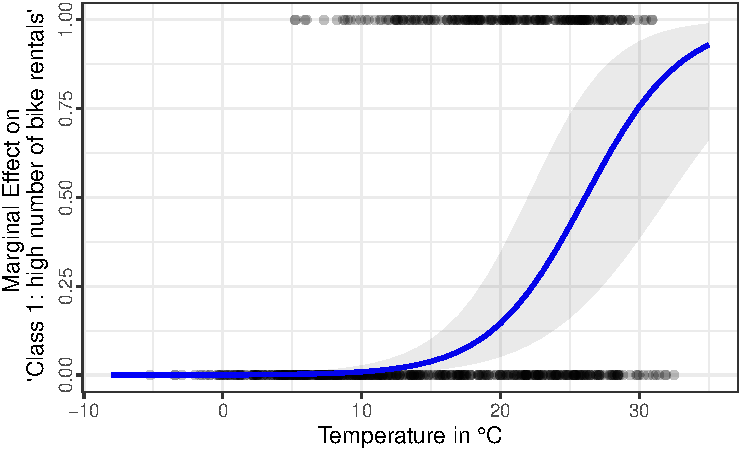
\includegraphics[width = 0.9\textwidth]{figure/logistic_marginal_temp.pdf}
\end{column}
\end{columns}

\bigskip

\textbf{Interpretation}
\begin{itemize}
    %\item If the temperature increases by 1 degree Celsius then the log odds of high number of bike rentals increase linearly by 0.3 c.p.
    \item If \code{temp} increases by 1$^\circ C$, odds ratio for class 1 increases by factor $\exp (0.29) = 1.34$ compared to class 0, c.p. ($\hat =$ ``high number of bike rentals'' now 1.34 times more likely)
    %\item If \code{season} is SPRING instead of WINTER (reference), odds ratio for class 1 increases by factor $\exp (1.74) = 1.34$ compared to class 0
\end{itemize}
\end{frame}

%------------------------------------------------------------------
%------------------------------------------------------------------

\endlecture
\end{document}
